% !TEX encoding = UTF-8 Unicode

\documentclass[a4paper,12pt, norsk]{article}
\usepackage[utf8]{inputenc}
\usepackage{graphicx}
\usepackage[norsk]{babel}
\usepackage{parskip}






\title{KTN1 \\ Prosjektplan}
\author{Fellesprosjektet: Gruppe 27 \\ Andreas Drivenes, Bjørn Bråthen, Nicholas Tidemann, \\ Eivind Gjerde Johansen, Eivind Havikbotn, Einar Eilertsen Eldevik}
\date{3. mars 2014}
\begin{document}
\maketitle

\section*{Klassediagram}
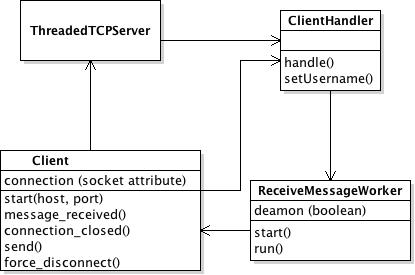
\includegraphics{klassediagram.jpg}

\clearpage


\section*{Sekvensdiagram}

\begin{figure}[!htb]
\centerline{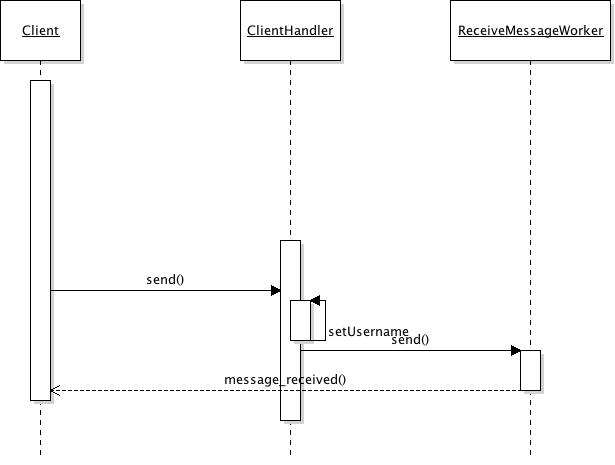
\includegraphics[scale=0.75]{login}}
\caption{Login}
\label{fig:lgoin}
\end{figure}

\begin{figure}[!htb]
\centerline{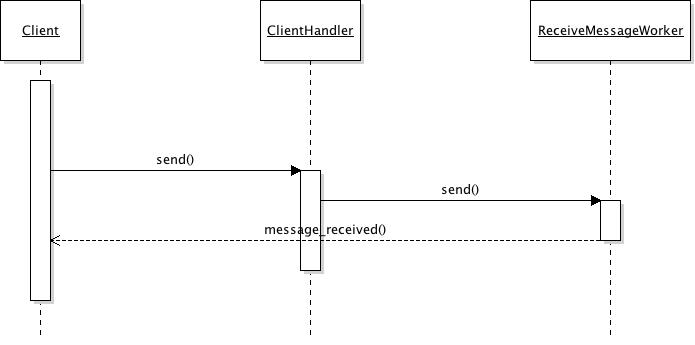
\includegraphics[scale=0.75]{send}}
\caption{Send}
\label{fig:send}
\end{figure}

\begin{figure}[!htb]
\centerline{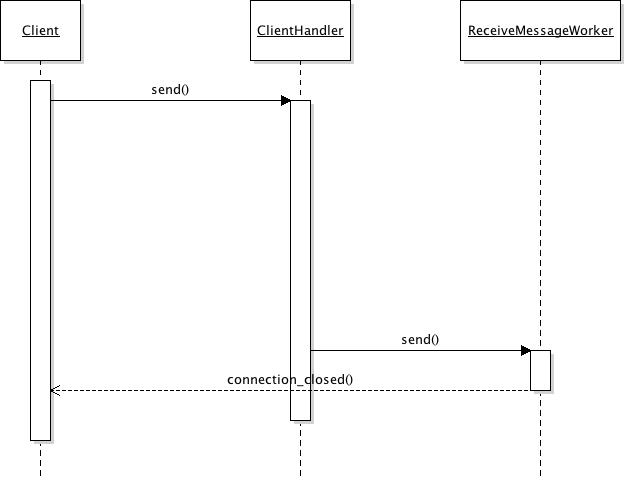
\includegraphics[scale=0.75]{logout}}
\caption{Logout}
\label{fig:logout}
\end{figure}

\clearpage



\section*{Tekstlig beskrivelse av design}
ThreadedTCPServer kan behandle flere brukere samtidig ved hjelp av ClientHandler. handle-metoden kjøres en gang per klient som kobler seg på. Serverobjektet må lagre en liste med brukernavn slik at den kan sjekke om brukernavnet er tatt. Den må også lagre en liste over alle meldingene denne sesjonen slik at denne kan broadcastes til en klient som logger seg på. 

For at det skal være mulig å motta og sende data samtidig for klienten, har vi ReceiveMessageWorker-tråden som lytter på meldinger fra serveren. Da kan en melding skrevet av en annen klient mottas samtidig som "vår" klient sender en annen melding. Den fungerer altså som et mellomlag mellom klient og server. ReceiveMessageWorker oppretter man som et trådobjekt i start-metoden til Client. Dette objektet kan så kalle på metoder i klient siden den tar inn et Client-objekt som lytter. 

Client-klassen vår sender data direkte til serveren. Kommunikasjonen skjer ved hjelp av JSON-objekter, og må implementeres som det står i protokollen på server- og klient-side.



\end{document}
